%Before characterizing a fiber several tasks had to be performed to check that the system is working properly. The quality of the tightness to the light of the black box used and the correct operation of the PMT for this study, which involves checking the correct operation of the PCB designed and checking the linearity of the PMT output signal in the study range, must be verified.

Before characterizing a fiber several tasks had to be performed to check that the black box was light-tight and the PMT response was lineal.

%First, the quality of the light tightness of the black box used was verified. It is important because we are detecting small signals, a few hundred photons per nanosecond, so it must be verified that the background of the system are below that.

A light leak in the black box would produce a background larger than the signal. To check the light-tightness a no-clad fiber of $20~\cm$ length was fixed in the previous assembly. The LED was fed with four different intensities ($0.05~\milli\ampere$, $0.1~\milli\ampere$, $0.15~\milli\ampere$ and $0.2~\milli\ampere$) and the PMT response was measured with and without a special black blanket from Thorlabs \cite{BlackBlancket}, that prevents external photons to reach the system. 

This test was repeated for three different fibers and the mean and standard deviation of the light output were calculated by:

\begin{equation}
\bar{x}=\frac{\sum_{i=0}^{N}x_i}{N}; \qquad \sigma = \frac{\sqrt{\sum_{i=0}^{N}(x_i-\bar{x})^2}}{N-1};
\label{eq:MeanAndStandardDesviation}
\end{equation}

The difference of the PMT responses in both cases is presented in Figure \ref{fig:LightTightnessTest}. As it can be seen in this figure, there are no statistically relevant differences between covered and uncovered fiber. Therefore, the light tightness of the black box is sufficient for this study.


%\begin{figure}[]
 %\centering
  %\subfloat[The measurement obtained by covering the setup with a special black blanket and not covering.]{
   %\label{subfig:LightTightnessTestData}
    %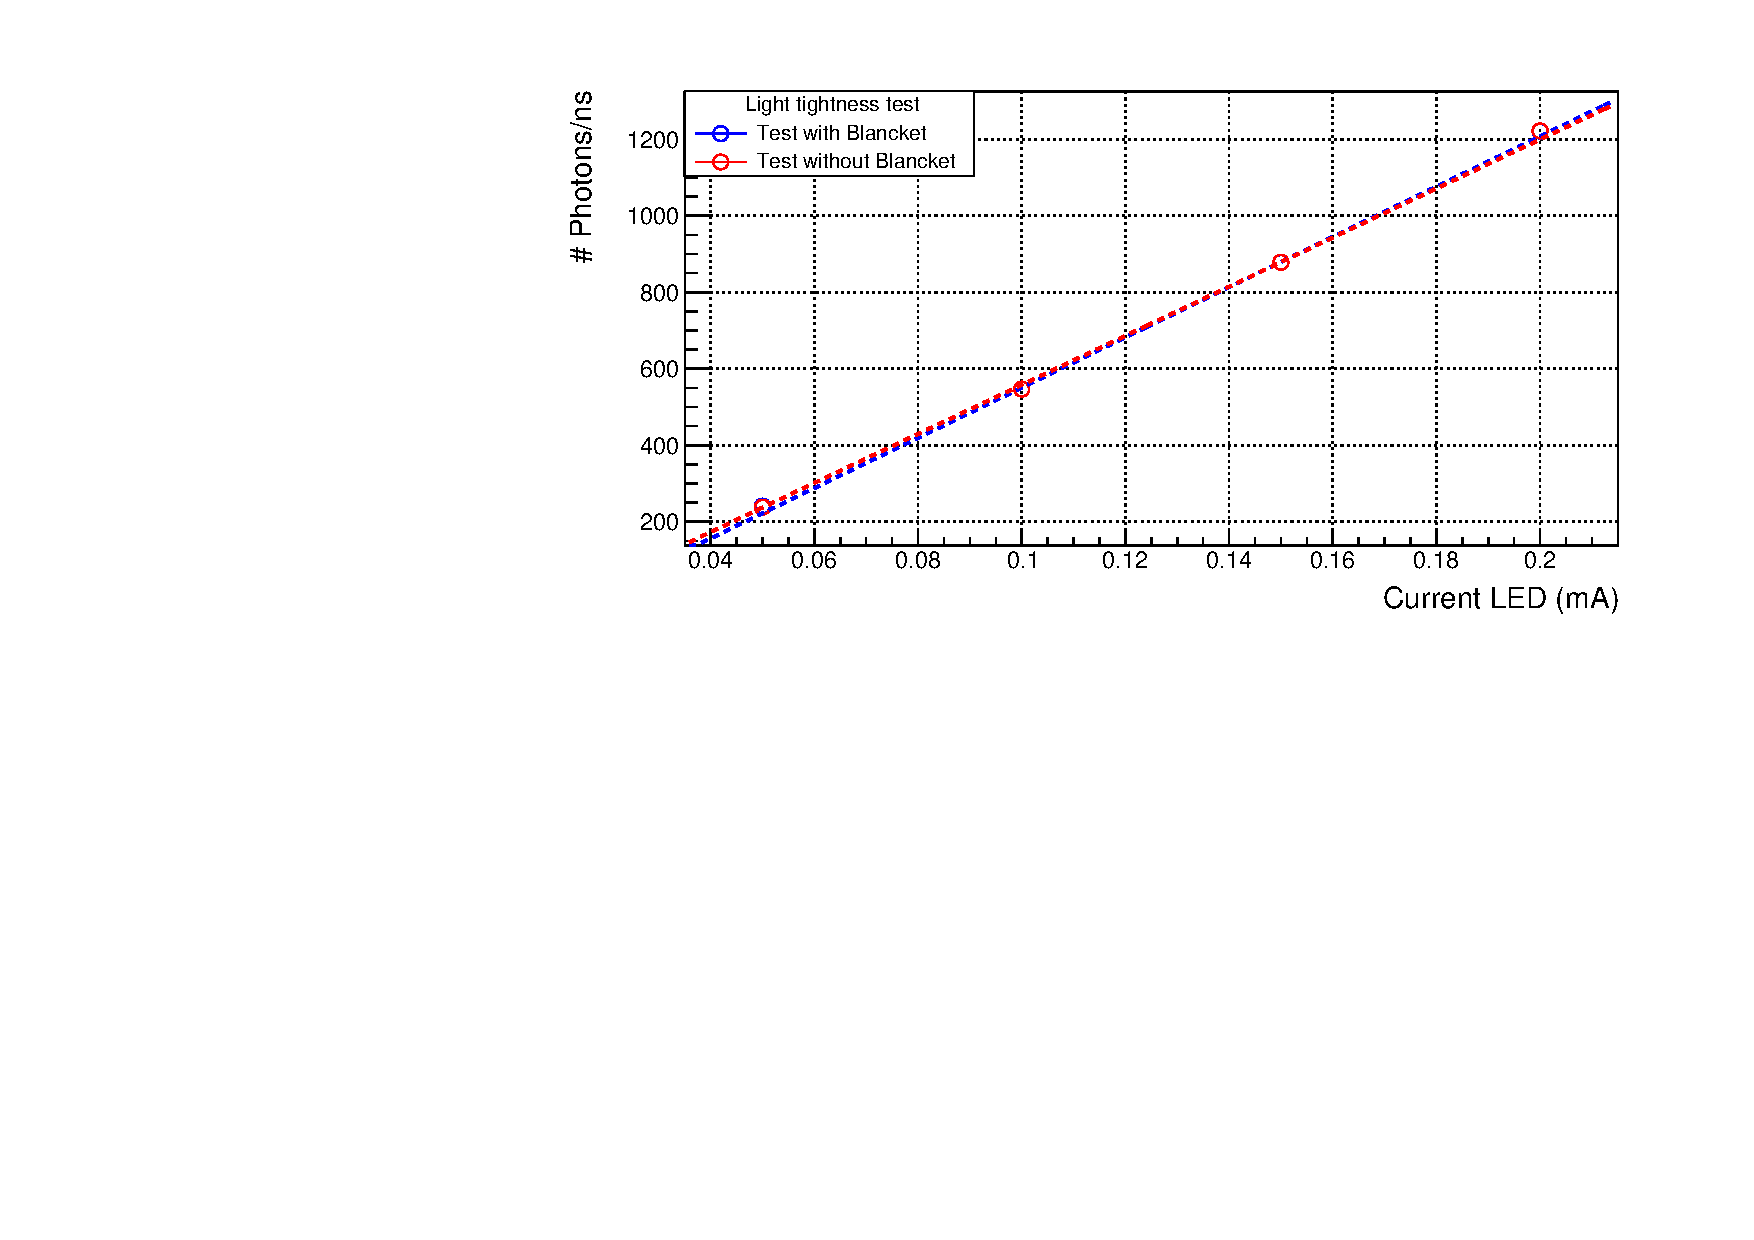
\includegraphics[width=0.9\textwidth]{4ResearchAndDevelopments/41Fibers/Light_tightness_Measurements.pdf}}
    %\newline
  %\subfloat[.]{
   %\label{subfig:LightTightnessTestDifference}
    %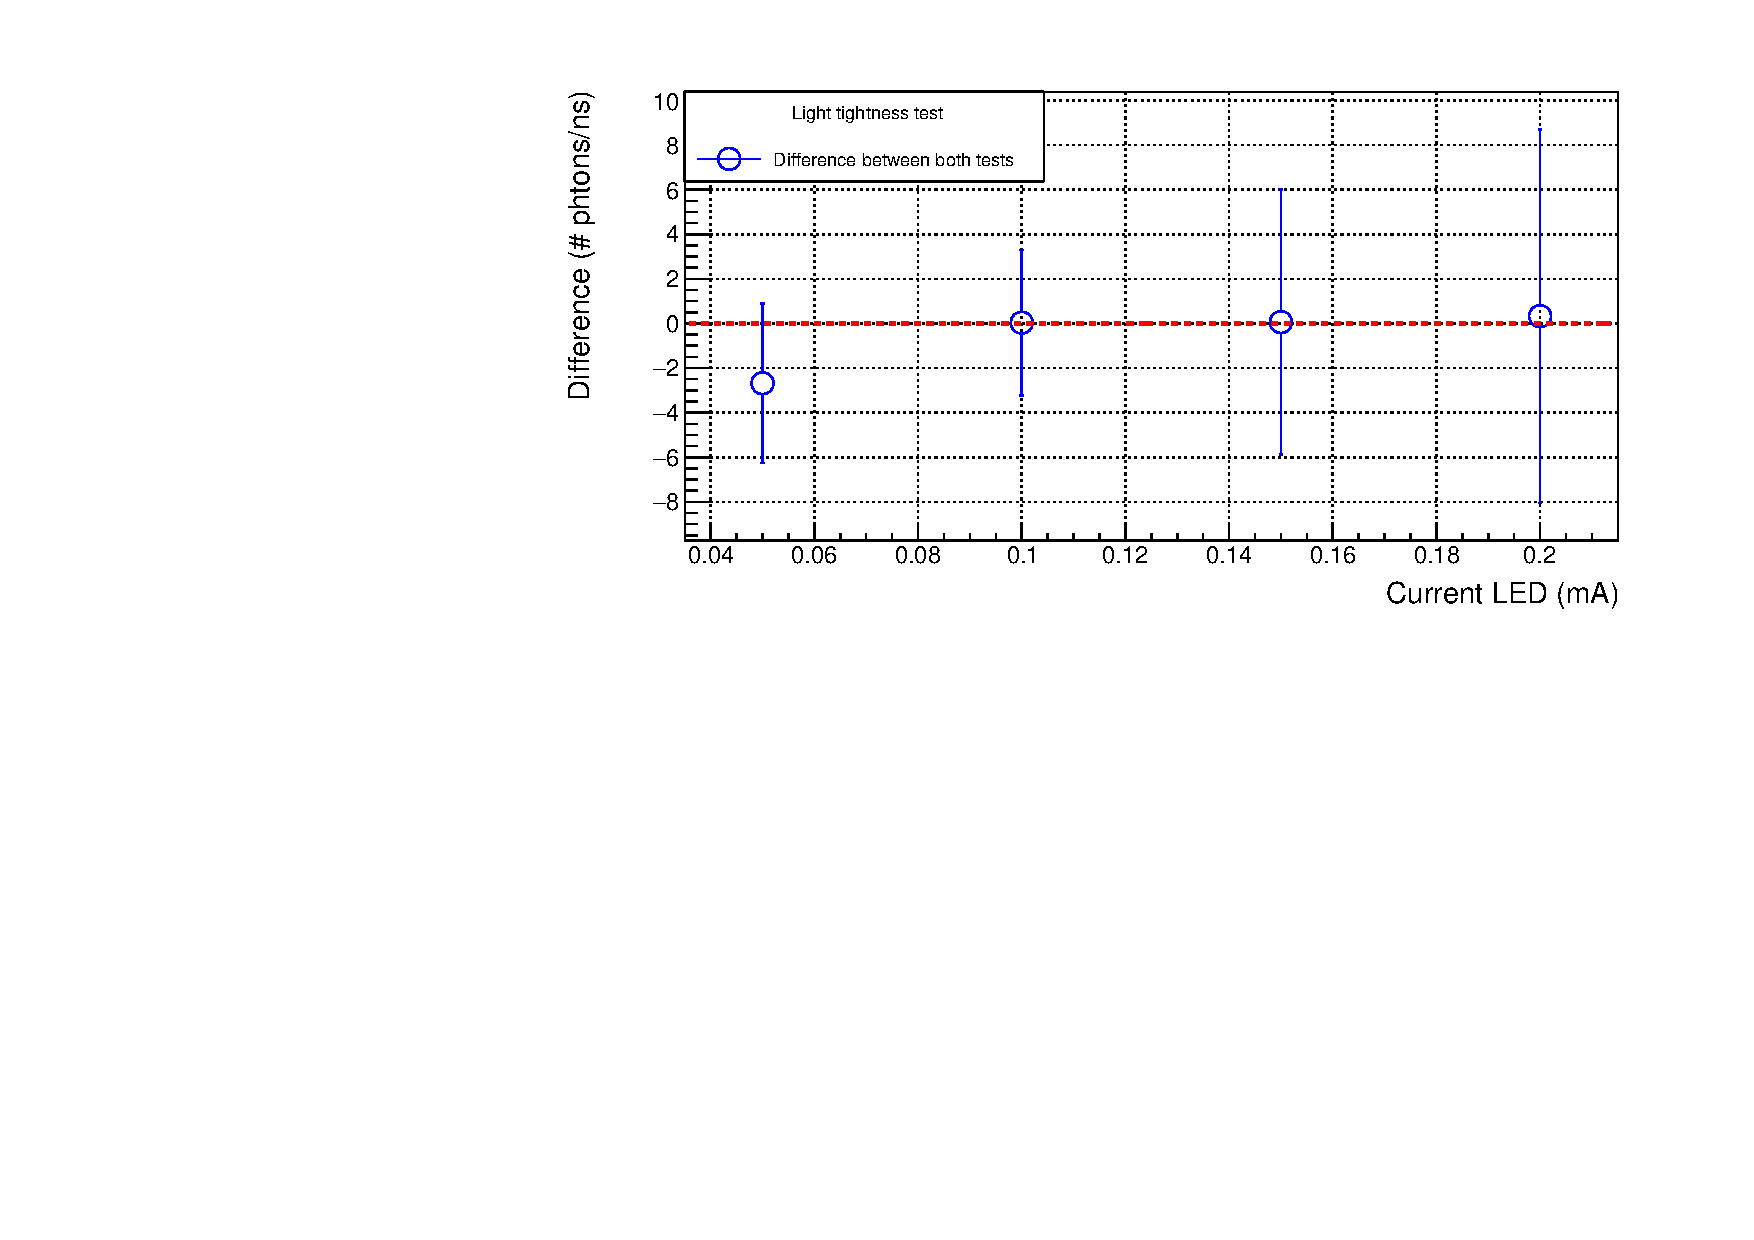
\includegraphics[width=0.9\textwidth]{4ResearchAndDevelopments/41Fibers/Light_tightness_difference.pdf}}
 %\caption{Energy spectrums used to test the effect of the Polishing machine}
 %\label{fig:LightTightnessTest}
%\end{figure}

\begin{figure}[h]
\centering
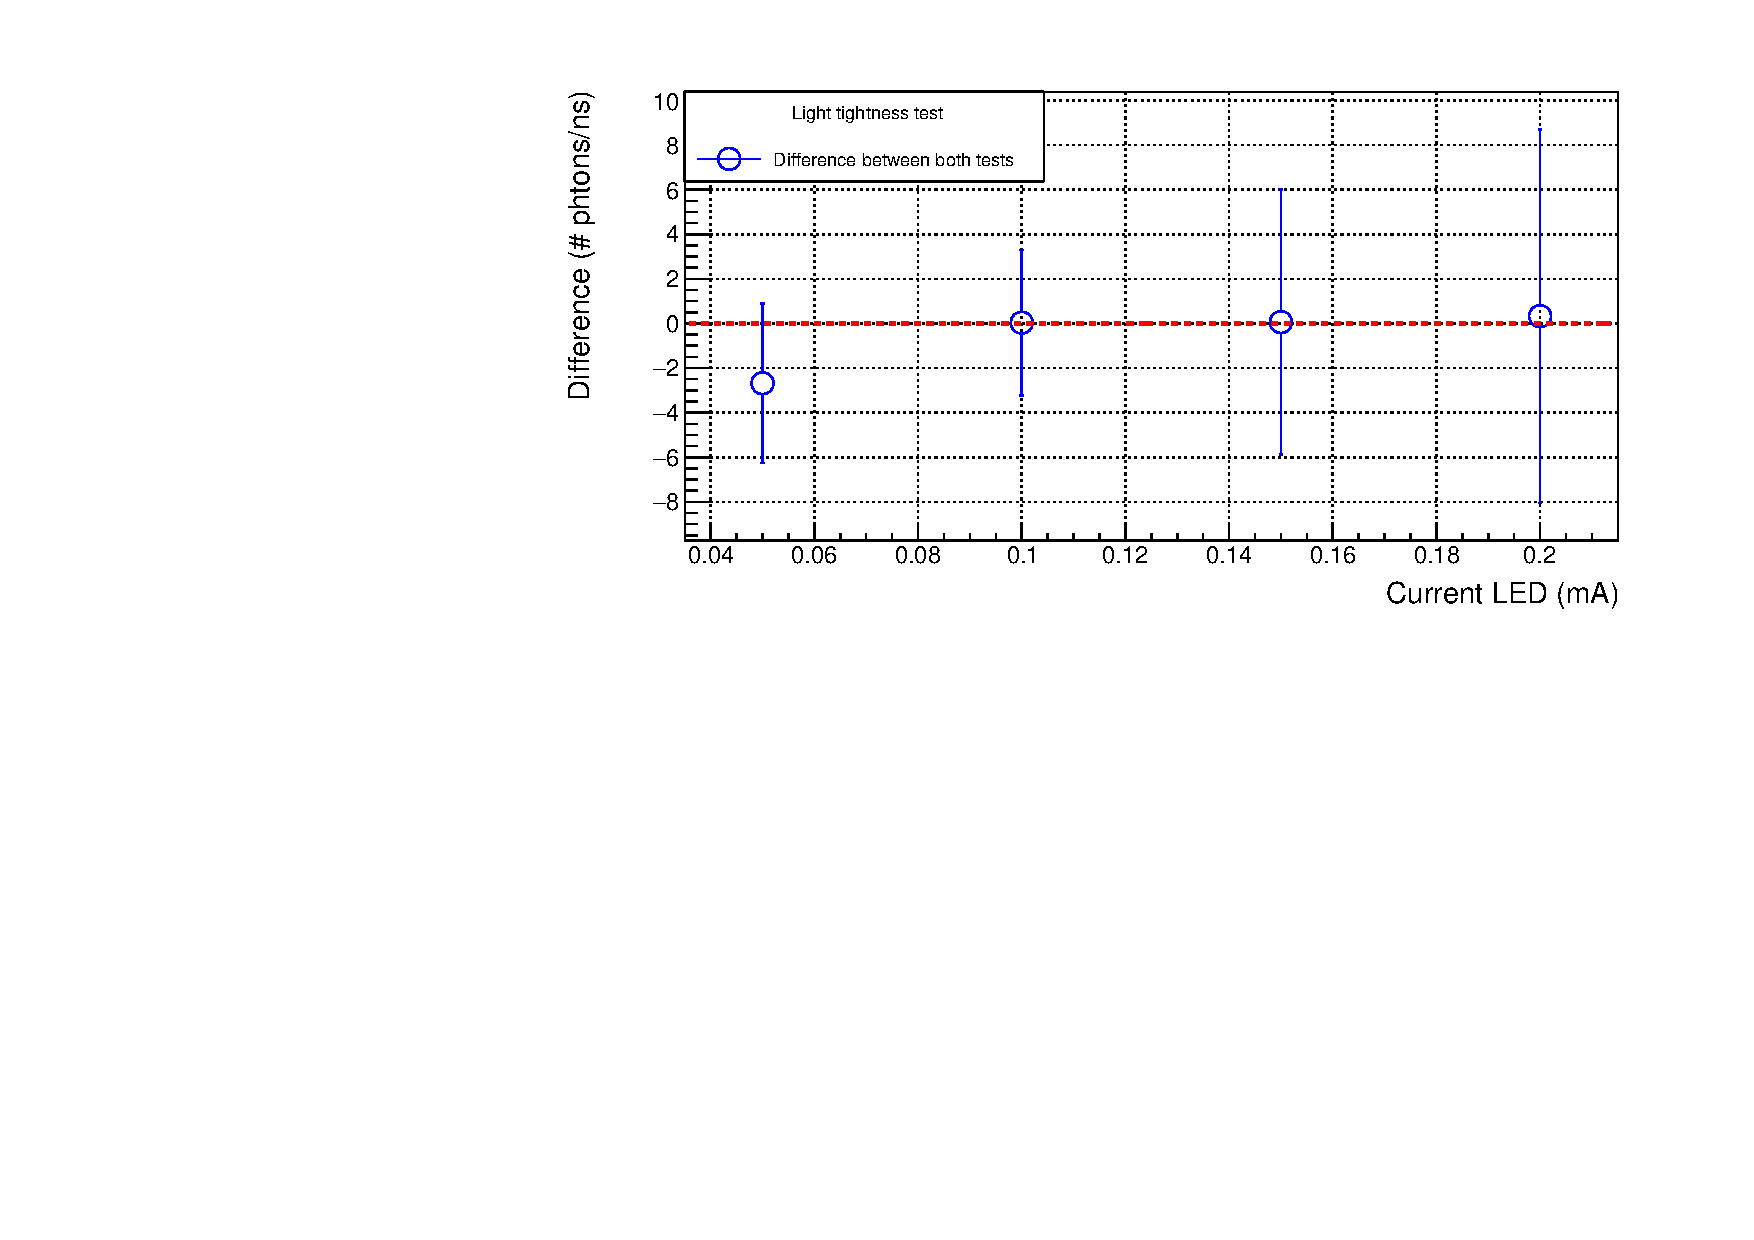
\includegraphics[scale=0.6]{4ResearchAndDevelopments/41Fibers/Light_tightness_difference.pdf}
\caption{Difference between the results obtained in both tests carried out to check the light-tight quality of the system.\label{fig:LightTightnessTest}}
\end{figure}

The optimal voltage of the PCB without the internal gain was obtained by finding the voltage plateau in which the electron collection efficiency in the first dynode was practically $100\%$. The LED was fed at $1~\milli\ampere$ intensity without any fiber and the PMT output current was measured for different PMT supply voltages, between $0$ and $500~\volt$. The number of photons detected by the PMT is plotted in Figure \ref{fig:PlateauNoGainPMT}. As it can be seen, the plateau is located at voltages higher than $150~\volt$, where the PMT output response is stable. The chosen voltage at which the characterization was carried out was $250~\volt$.


\begin{figure}[h]
\centering
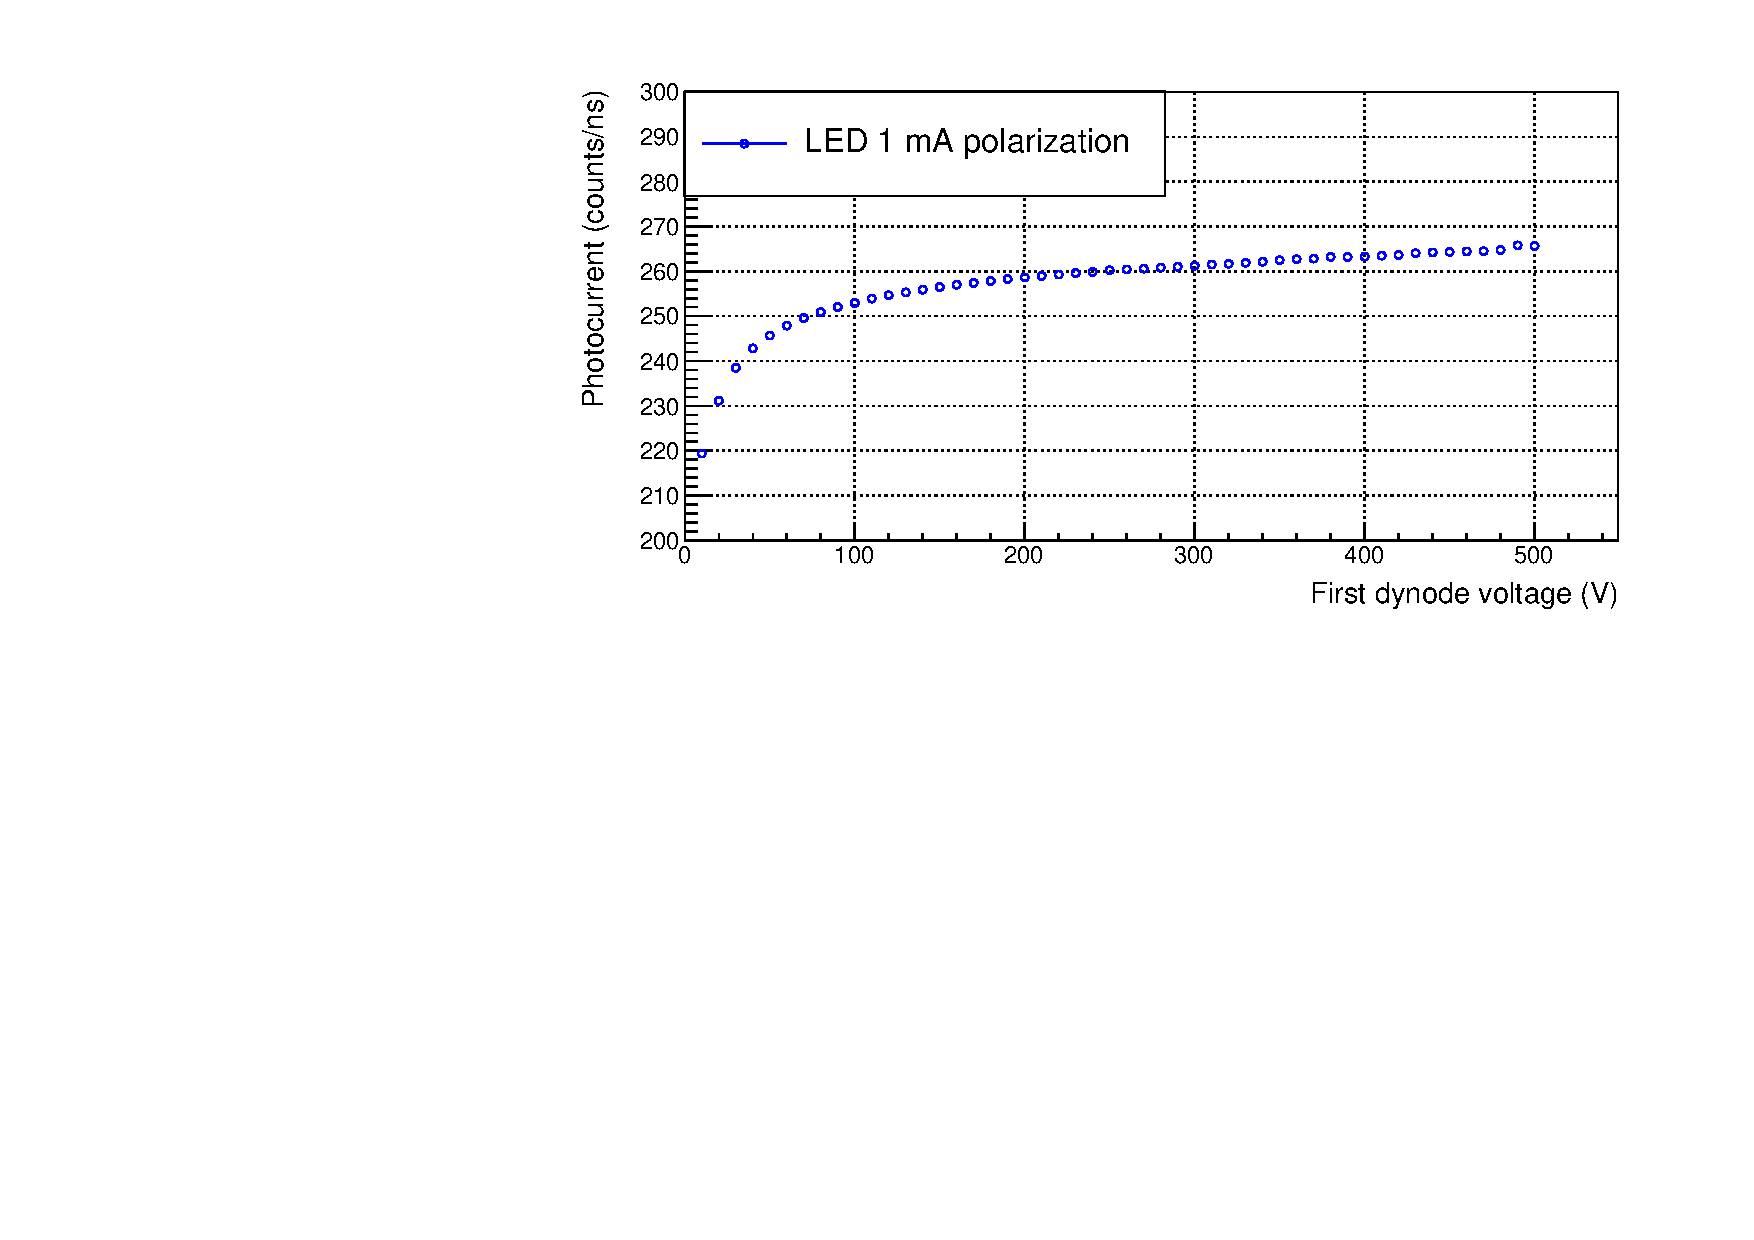
\includegraphics[scale=0.6]{4ResearchAndDevelopments/41Fibers/PCBNoGainPlateau_Calibrated.pdf}
\caption{Response of the PMT as a function of its high voltage using the designed PCB with which no internal gain of the PMT is obtained.\label{fig:PlateauNoGainPMT}}
\end{figure}

Finally, the linearity of the PMT was verified. The LED was powered with intensities ranging from 0 to $10~\milli\ampere$ (LED linearity range) to check that the LED emission light do not saturate. The linearity was tested in the range of the number of photons expected in a tritium event (a few tens of photons per tritium event, tens of photons per nanosecond) and in the range of up to two thousand five hundred photons per nanosecond.

To test the linearity of the PMT in the range of tritium events, the set up described above was used without any fiber and one of the connectors but the collimators was kept to make sure that the active area of the PMT is the same as the use in the characterization study.

To test the linearity of the PMT at the level of more than a thousand photons per nanosecond, we removed the remaining connector in order to increase the photons that reach the photosensor and the collimators was also kept.

The results for both intensity ranges are shown in Figures \ref{fig:LinearityRangesOfPMT}. As it can be seen, the PMT output current is linear in both intensity ranges.

\begin{figure}
\centering
    \begin{subfigure}[b]{0.8\textwidth}
    \centering
    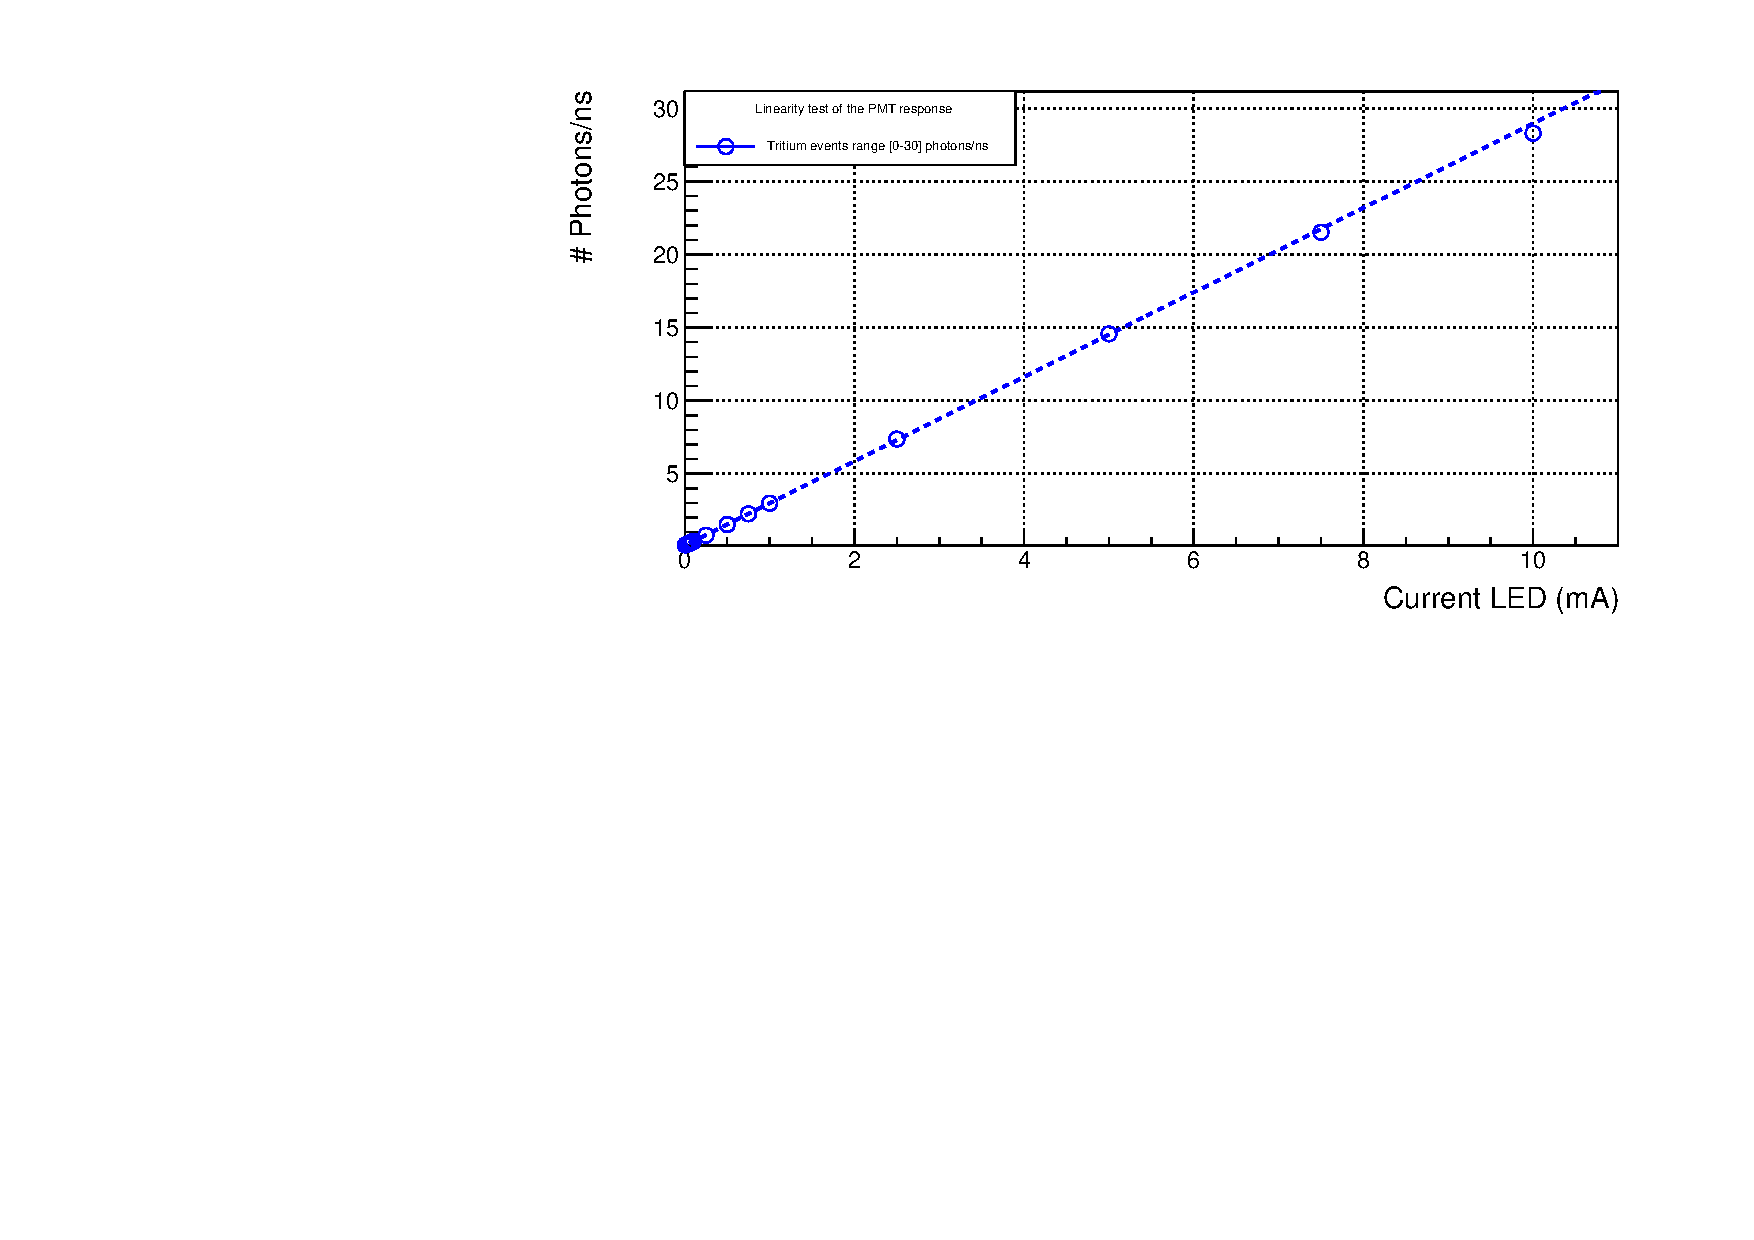
\includegraphics[width=\textwidth]{4ResearchAndDevelopments/41Fibers/Linearity_test_0_30_range.pdf}  
    \caption{Verification of linearity in the response of the PMT in the range of tritium events.\label{subfig:LinearityTritiumRange}}
    \end{subfigure}
    \hfill
    \begin{subfigure}[b]{0.8\textwidth}
    \centering
    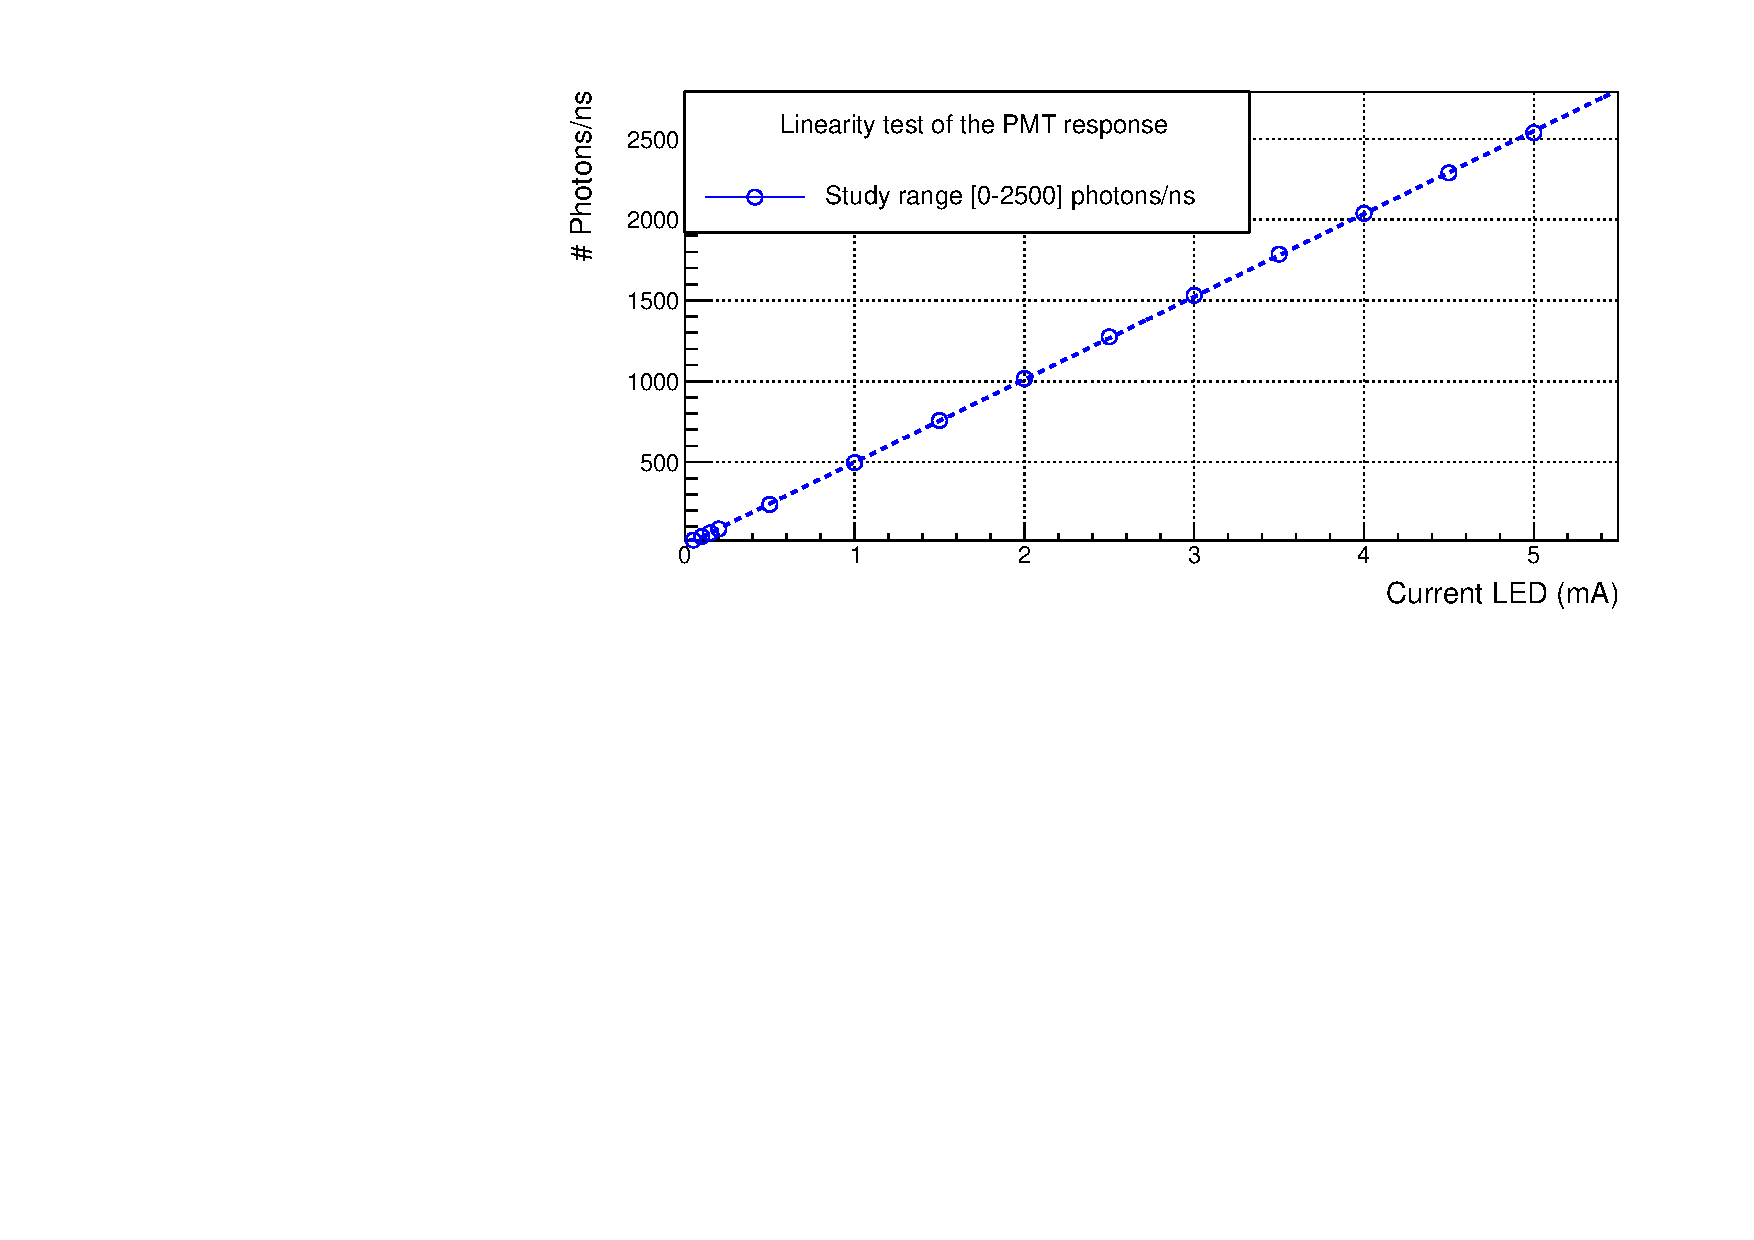
\includegraphics[width=\textwidth]{4ResearchAndDevelopments/41Fibers/Linearity_test_0_2500_range.pdf}  
    \caption{Verification of linearity in the response of the PMT in the range of this study  $(0-2500)~\gamma/\nano\second$.\label{subfig:LinearityStudyRange}}
    \end{subfigure}
 \caption{Linearity tests of the PMT response}
 \label{fig:LinearityRangesOfPMT}
\end{figure}